% Fig. 1: block diagram of the proposed control scheme (one-column width).
% Compile with pdflatex to obtain figs/fig_block_proposed_afc.pdf.
\documentclass[border=1pt]{standalone}
\usepackage{mathptmx}
\usepackage{amsmath}
\usepackage{tikz}
\usetikzlibrary{arrows.meta,calc}
\begin{document}
\footnotesize
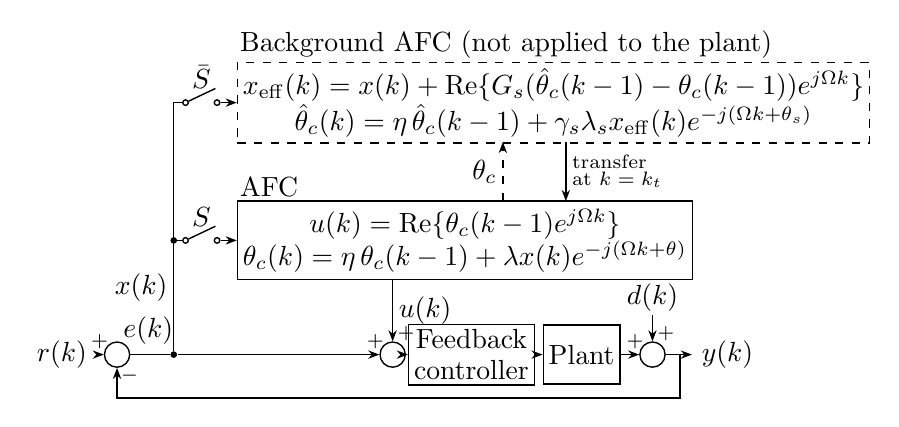
\begin{tikzpicture}[
  >={Stealth[length=4pt,width=3pt]},
  line width=0.5pt,
  blk/.style={draw,minimum height=7.5mm,align=center,inner sep=2pt},
  sum/.style={draw,circle,inner sep=0pt,minimum size=3.2mm},
  dot/.style={circle,fill,inner sep=0pt,minimum size=2.4pt},
  sw/.style={circle,draw,fill=white,inner sep=0pt,minimum size=2pt},
  sgn/.style={font=\scriptsize,inner sep=0pt},
]
% coordinates
\def\xb{1.42}   % branch line of x(k)
\def\ya{1.45}   % AFC
\def\yb{3.20}   % background AFC

% ---------------- main loop (bottom) ----------------
\node (r) at (0,0) {$r(k)$};
\node[sum] (s1) at (0.70,0) {};
\node[dot] (ne) at (\xb,0) {};
\node[sum] (s2) at (4.20,0) {};
\node[blk,minimum width=13mm] (C) at (5.20,0) {Feedback\\[-1pt]controller};
\node[blk,minimum width=9mm] (P) at (6.60,0) {Plant};
\node[sum] (s3) at (7.50,0) {};
\node[anchor=west] (y) at (8.00,0) {$y(k)$};
\draw[->] (r) -- (s1);
\draw (s1) -- (ne);
\node[above,inner sep=2pt] at ($(s1)!0.55!(ne)+(0,0.05)$) {$e(k)$};
\draw[->] (ne) -- (s2);
\draw[->] (s2) -- (C);
\draw[->] (C) -- (P);
\draw[->] (P) -- (s3);
\draw[->] (s3) -- (y);
\draw[->] (7.85,0) -- (7.85,-0.55) -- (0.70,-0.55) -- (s1);
\node[sgn] at (0.48,0.16) {$+$};
\node[sgn] at (0.86,-0.27) {$-$};
\node[sgn] at (3.98,0.16) {$+$};
\node[sgn] at (4.37,0.27) {$+$};
\draw[<-] (s3) -- ++(0,0.50) node[above,inner sep=1pt] {$d(k)$};
\node[sgn] at (7.28,0.16) {$+$};
\node[sgn] at (7.67,0.27) {$+$};

% ---------------- AFC (middle) ----------------
\node[blk,anchor=west,minimum height=10mm] (afc) at (2.22,\ya)
  {$u(k)=\operatorname{Re}\{\theta_c(k-1)e^{j\Omega k}\}$\\
   $\theta_c(k)=\eta\,\theta_c(k-1)+\lambda x(k)e^{-j(\Omega k+\theta)}$};
\node[anchor=south west,inner sep=1pt] at (afc.north west) {AFC};
\draw[->] (s2 |- afc.south) -- node[right,inner sep=2pt] {$u(k)$} (s2);

% ---------------- background AFC (top) ----------------
\node[blk,dashed,anchor=west,minimum height=10mm] (bg) at (2.22,\yb)
  {$x_\mathrm{eff}(k)=x(k)+\operatorname{Re}\{G_s(\hat{\theta}_c(k-1)-\theta_c(k-1))e^{j\Omega k}\}$\\
   $\hat{\theta}_c(k)=\eta\,\hat{\theta}_c(k-1)+\gamma_s\lambda_s x_\mathrm{eff}(k)e^{-j(\Omega k+\theta_s)}$};
\node[anchor=south west,inner sep=1pt] at (bg.north west) {Background AFC (not applied to the plant)};

% coefficient paths between the two AFCs
\draw[->,dashed] (5.60,\ya+0.5) -- node[left,inner sep=2pt] {$\theta_c$} (5.60,\yb-0.5);
\draw[->] (6.40,\yb-0.5) -- node[right,inner sep=2pt,align=left,font=\scriptsize]
  {transfer\\[-2pt]at $k=k_t$} (6.40,\ya+0.5);

% ---------------- input branch with switches ----------------
\draw (ne) -- (\xb,\yb) -- (\xb+0.12,\yb);
\draw (\xb,\ya) -- (\xb+0.12,\ya);
\node[dot] at (\xb,\ya) {};
\node[left,inner sep=2pt] at (\xb,0.85) {$x(k)$};
% switch S (AFC)
\node[sw] (a1) at (\xb+0.15,\ya) {};
\node[sw] (a2) at (\xb+0.55,\ya) {};
\draw (a1) -- ++(0.38,0.18);
\node[above,inner sep=2pt] at (\xb+0.35,\ya+0.1) {$S$};
\draw[->] (a2) -- (afc.west);
% switch S-bar (background AFC)
\node[sw] (b1) at (\xb+0.15,\yb) {};
\node[sw] (b2) at (\xb+0.55,\yb) {};
\draw (b1) -- ++(0.38,0.18);
\node[above,inner sep=2pt] at (\xb+0.35,\yb+0.1) {$\bar{S}$};
\draw[->] (b2) -- (bg.west);
\end{tikzpicture}
\end{document}
